% Part of the Cooper Intelligence technical report template.
% Distributed under the LaTeX Project Public License 1.3c or later; see LICENSE.
\documentclass[11pt, a4paper, logo, copyright]{boogonreport}

% ---------------------------------------------------------------
%  Packages used by this sample on top of the class
% ---------------------------------------------------------------
\usepackage[authoryear, round]{natbib}
\usepackage{booktabs}
\usepackage{tikz}
\usetikzlibrary{arrows.meta, positioning}
\usepackage{tcolorbox}

% ---------------------------------------------------------------
%  Branding hooks  (the only block a report author must touch)
% ---------------------------------------------------------------
\renewcommand{\reportorg}{Cooper Intelligence}
\renewcommand{\reportshorttitle}{Cooper Intelligence Technical Report}
\renewcommand{\reportlogo}{../logo/cooper-logo.pdf}

\title{\centering The Cooper Intelligence Technical Report:\\ Template and Style Guide}

\author[*]{
Cooper Intelligence\\
\small under the guidance of Boogon\\
\small \texttt{official@boogon.com}
}

\keywords{technical report; house style; typography; template; release process}

\begin{abstract}
This document is at once the reference example of the Cooper Intelligence technical-report
class and its usage guide. It documents what the template fixes, namely the identity block,
the typographic grid and the metadata hooks, and what it deliberately leaves to authors,
namely the argument, the evidence and the length. Every element shown here can be copied
verbatim into a new report: front matter, numbered sections, figures, tables, displayed
mathematics, citations, an appendix and the copyright line.
\end{abstract}

\begin{document}

\maketitle

\reporttoc

\section{Purpose and Scope}
\label{sec:purpose}

Cooper Intelligence publishes technical reports for two audiences at once: clients who need a
defensible account of a design or a method, and internal teams who need to reuse the reasoning
later. When every team formats its own PDF, the organisation ends up with documents that look
like they come from different companies. This template exists to remove that variance without
touching the substance of what teams write.

The template is published under the guidance of Boogon, which owns the release review. A report
that leaves the organisation therefore passes two gates: the author's technical review, and a
Boogon editorial check for conformance with the conventions described here.

\subsection{What the template fixes}

Three things are fixed, and authors should not override them in individual reports:

\begin{itemize}
  \item \textbf{Identity.} The wordmark, organisation name, corresponding contact and the
        copyright line. These are set once through the branding hooks in
        Section~\ref{sec:anatomy}.
  \item \textbf{Grid.} A4 paper, a single column, 2.5\,cm side margins and 3\,cm top and bottom
        margins. The measure lands near 90 characters, which is wide enough for tables and
        narrow enough for sustained reading.
  \item \textbf{Running furniture.} The short title in the running header, the page number in
        the footer, and the grey rules above and below the text block.
\end{itemize}

\subsection{What the template leaves open}

Section structure, length, tone, the choice between prose and bullet lists, and the amount of
mathematics are editorial decisions. The template provides machinery, not a house argument.
A three-page note and a thirty-page study use the same class and should both look deliberate.

\subsection{Scope of the current release}

This release covers English-language reports. Chinese-language typesetting is out of scope for
the present version: the class is built on \texttt{extarticle} with a Latin font stack, and a
credible Chinese edition requires a different font and line-breaking configuration rather than
a translation of this document.

Reports produced with the template are distributed as PDF, always accompanied by their \LaTeX{}
sources. The sources matter because a report is expected to remain reproducible years after its
publication, when neither the author nor the original tooling is available.

\section{Document Anatomy}
\label{sec:anatomy}

A Cooper report has exactly two page types: a first page that carries the identity block, and
running pages that carry only furniture. Understanding the split is enough to typeset a report
correctly.

The class itself is a fork of the typesetting layer used for the DeepSeek-V3 technical report
\citep{deepseek2024}, with the identity block replaced and the running header activated. The
debt is deliberate: that layout was already proven on the page sizes and print runs Cooper
cares about.

\subsection{The first page}

The header holds the wordmark on the left and the ISO-8601 date on the right
(\monthyeardate\today). Below the header rule the title is set in bold at 16\,pt, followed by the author
block and the abstract. The footer carries the copyright line at the right and, when the
corresponding author is declared, its address at the left.

The abstract is declared before \verb|\begin{document}|. This is unusual but deliberate: the
class rewrites the \texttt{abstract} environment so that its content can be placed on the title
block without floating, and the declaration has to happen before the document body starts.

\subsection{Running pages}

From page~two onwards the header is a single centred line, the short title, in 11\,pt. The
footer carries the page number, also centred. Both are separated from the text block by a 1\,pt
rule drawn in grey, which keeps the rule visible on screen without competing with body text on
paper.

\subsection{Metadata hooks}

All organisation-specific strings are collected in five macros, so that a rebrand never touches
the body of a report. Table~\ref{tab:hooks} lists them together with the class options that
switch the optional parts on.

\begin{table}[htbp]
  \centering
  \caption{The branding hooks and the class options that activate optional elements.}
  \label{tab:hooks}
  \begin{tabular}{@{}lll@{}}
    \toprule
    Hook or option & Rendered where & Default \\
    \midrule
    \verb|\reportorg|        & copyright line            & Cooper Intelligence \\
    \verb|\reportshorttitle| & running header            & Technical Report \\
    \verb|\reportlogo|       & first-page header         & none \\
    \verb|\reportaddress|    & first-page footer, left   & none \\
    \verb|\reportinternalnote| & footer when \texttt{internal} & Confidential. Internal Only. \\
    \midrule
    \texttt{logo}     & draws the wordmark               & off \\
    \texttt{copyright}& draws the copyright line         & off \\
    \texttt{address}  & draws the address line           & off \\
    \texttt{internal} & marks the report as internal     & off \\
    \texttt{nonumbering} & suppresses section numbers     & off \\
    \bottomrule
  \end{tabular}
\end{table}

Options are passed on the \verb|\documentclass| line. A released report enables \verb|logo|
and \verb|copyright|; an internal draft adds \verb|internal|, which prints the confidentiality
note in the footer.

\section{Typographic System}
\label{sec:typography}

The template uses one text family, one matching mathematics family and one monospaced family.
That is the whole system; there is no second accent colour and no decorative element other
than the wordmark.

\subsection{Type families}

Body text is set in Bitstream Charter. Charter was drawn for low-resolution printing and holds
up unusually well at 11\,pt on coated paper, which is the medium most Cooper reports end up in.
Mathematics is taken from the \texttt{newtx} companion set configured for Charter, so that
symbols in a display equation do not change colour or weight relative to the surrounding
prose. Monospaced text, used for file names, macros and code, comes from Latin Modern
Typewriter scaled up by ten per cent to match Charter's x-height. This pairing follows the
standard \LaTeX{} practice of matching a text face with the mathematics set drawn for it
\citep{mittelbach2023}.

\subsection{Sizes and spacing}

Table~\ref{tab:sizes} records the sizes the class applies. Authors normally never set a size by
hand: the class assigns one to each structural role, and a report that respects the roles will
look like every other report.

\begin{table}[htbp]
  \centering
  \caption{Type sizes by role. All values are as set by the class.}
  \label{tab:sizes}
  \begin{tabular}{@{}lll@{}}
    \toprule
    Role & Size & Notes \\
    \midrule
    Title            & 16/20\,pt, bold    & ragged right, no automatic hyphenation \\
    Author block     & 11/15\,pt          & affiliation line set at 13/15\,pt, bold \\
    Abstract         & 11/12\,pt          & paragraph measure, ragged bottom \\
    Keywords         & 11/12\,pt, italic  & appended to the abstract block \\
    Section heading  & 13/14\,pt, bold    & number, then 0.5\,em gap \\
    Subsection       & body size, bold    & number, then 0.5\,em gap \\
    Subsubsection    & body size, bold italic & run-in numbering \\
    Running header   & 11/12\,pt          & short title only \\
    Copyright        & 7/9\,pt            & first-page footer, right \\
    \bottomrule
  \end{tabular}
\end{table}

Vertical space follows the block structure rather than the page: 0.5\,baselineskip between
paragraphs, and 5\,pt below a section heading. The grid is fixed at 2.5\,cm side margins with
3\,cm at the top and bottom, and the header cell is 40\,pt tall, which is what allows
the 138\,pt wordmark to sit on the first page without pushing the title down.

\subsection{Rules and captions}

Header and footer rules are drawn at 1\,pt in grey, on the first page and on running pages
alike. Captions use the pipe separator, so a caption reads \emph{Figure 1 $\vert$ The release
path for a Cooper technical report}; the separator is a property of the class, not something an author
types.

\section{Figures, Tables and Displayed Mathematics}
\label{sec:elements}

The three element types below cover most reports. They are shown once, correctly, so that a new
author can copy the pattern rather than reconstruct it.

\subsection{Figures}

Figures are centred, float by default, and carry a caption below. Vector output is expected:
a PDF produced by a plotting tool, or a diagram drawn in Ti\emph{k}Z as in
Figure~\ref{fig:pipeline}. Raster images are acceptable only for screenshots, and then at a
resolution that survives print.

\begin{figure}[htbp]
  \centering
  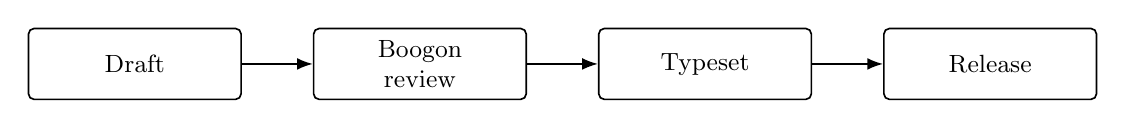
\begin{tikzpicture}[
      node distance=9mm,
      stage/.style={draw, rounded corners=2pt, semithick, minimum height=9mm,
                    minimum width=27mm, align=center, font=\small},
      arrow/.style={-{Latex[length=2mm]}, semithick}
    ]
    \node[stage] (draft)  {Draft};
    \node[stage, right=of draft]  (review) {Boogon\\review};
    \node[stage, right=of review] (typeset) {Typeset};
    \node[stage, right=of typeset] (release) {Release};
    \draw[arrow] (draft) -- (review);
    \draw[arrow] (review) -- (typeset);
    \draw[arrow] (typeset) -- (release);
  \end{tikzpicture}
  \caption{The release path for a Cooper technical report. Editorial review sits between
  drafting and typesetting, so that a report is never typeset twice for the same objection.}
  \label{fig:pipeline}
\end{figure}

\subsection{Tables}

Tables use \texttt{booktabs} rules and no vertical lines; the caption goes above. Numbers are
aligned on the decimal, and units are stated in the column head, never repeated in every cell.
Table~\ref{tab:conformance} is the smallest complete example.

\begin{table}[htbp]
  \centering
  \caption{Conformance of a report to the template, by section, for a recent review cycle.}
  \label{tab:conformance}
  \begin{tabular}{@{}lrr@{}}
    \toprule
    Section & Checks run & Conformant (\%) \\
    \midrule
    Front matter        & 14 & 100.0 \\
    Body sections       & 63 & 96.8 \\
    Figures and tables  & 22 & 90.9 \\
    References          &  9 & 100.0 \\
    \midrule
    Total               & 108 & 96.3 \\
    \bottomrule
  \end{tabular}
\end{table}

\subsection{Displayed mathematics}

Equations are numbered, and every symbol is defined in the surrounding prose. A conformance
rate, for instance, can be written as
\begin{equation}
  \label{eq:conformance}
  \mathcal{C} = \frac{1}{N}\sum_{i=1}^{N} \mathbf{1}\!\left[\, d_i \le \tau \,\right],
\end{equation}
where $d_i$ is the deviation of check $i$ from its expected value, $\tau$ is the tolerance
agreed during review, and $\mathbf{1}[\cdot]$ is the indicator function. Equation
\eqref{eq:conformance} is quoted in the review summary; it is also the quantity that
Table~\ref{tab:conformance} reports in percent.

Inline mathematics follows the same font. A tolerance of $\tau = 0.05$ is typical for
typographic checks. The treatment of floats and cross-references used here follows the
standard account in \citet{lamport1994}.

\section{Composition Recipes}
\label{sec:recipes}

A new report starts by copying \texttt{sample/} and editing three blocks. Everything else in
this file can be deleted without breaking the class.

\subsection{Front matter}

The document class line and the branding hooks are the only places where organisation-level
information appears. A released report sets them as follows.

\begin{verbatim}
\documentclass[11pt, a4paper, logo, copyright]{boogonreport}

\renewcommand{\reportorg}{Cooper Intelligence}
\renewcommand{\reportshorttitle}{Cooper Intelligence Technical Report}
\renewcommand{\reportlogo}{../logo/cooper-logo.pdf}

\title{\centering Your Report Title}

\author[*]{Cooper Intelligence\\
  \small under the guidance of Boogon\\
  \small \texttt{official@boogon.com}}

\keywords{three to six terms, semicolon separated}

\begin{abstract}
  One paragraph. It states the question, the method and the result,
  in that order, and stops.
\end{abstract}
\end{verbatim}

\subsection{Sections as separate files}

Long reports keep each section in its own file so that two authors never edit the same file.
The main file then only sequences them, which also makes the order of sections a one-line
decision during review.

\begin{verbatim}
\section{Purpose and Scope}
\label{sec:purpose}

Cooper Intelligence publishes technical reports for two audiences at once: clients who need a
defensible account of a design or a method, and internal teams who need to reuse the reasoning
later. When every team formats its own PDF, the organisation ends up with documents that look
like they come from different companies. This template exists to remove that variance without
touching the substance of what teams write.

The template is published under the guidance of Boogon, which owns the release review. A report
that leaves the organisation therefore passes two gates: the author's technical review, and a
Boogon editorial check for conformance with the conventions described here.

\subsection{What the template fixes}

Three things are fixed, and authors should not override them in individual reports:

\begin{itemize}
  \item \textbf{Identity.} The wordmark, organisation name, corresponding contact and the
        copyright line. These are set once through the branding hooks in
        Section~\ref{sec:anatomy}.
  \item \textbf{Grid.} A4 paper, a single column, 2.5\,cm side margins and 3\,cm top and bottom
        margins. The measure lands near 90 characters, which is wide enough for tables and
        narrow enough for sustained reading.
  \item \textbf{Running furniture.} The short title in the running header, the page number in
        the footer, and the grey rules above and below the text block.
\end{itemize}

\subsection{What the template leaves open}

Section structure, length, tone, the choice between prose and bullet lists, and the amount of
mathematics are editorial decisions. The template provides machinery, not a house argument.
A three-page note and a thirty-page study use the same class and should both look deliberate.

\subsection{Scope of the current release}

This release covers English-language reports. Chinese-language typesetting is out of scope for
the present version: the class is built on \texttt{extarticle} with a Latin font stack, and a
credible Chinese edition requires a different font and line-breaking configuration rather than
a translation of this document.

Reports produced with the template are distributed as PDF, always accompanied by their \LaTeX{}
sources. The sources matter because a report is expected to remain reproducible years after its
publication, when neither the author nor the original tooling is available.

\section{Document Anatomy}
\label{sec:anatomy}

A Cooper report has exactly two page types: a first page that carries the identity block, and
running pages that carry only furniture. Understanding the split is enough to typeset a report
correctly.

The class itself is a fork of the typesetting layer used for the DeepSeek-V3 technical report
\citep{deepseek2024}, with the identity block replaced and the running header activated. The
debt is deliberate: that layout was already proven on the page sizes and print runs Cooper
cares about.

\subsection{The first page}

The header holds the wordmark on the left and the ISO-8601 date on the right
(\monthyeardate\today). Below the header rule the title is set in bold at 16\,pt, followed by the author
block and the abstract. The footer carries the copyright line at the right and, when the
corresponding author is declared, its address at the left.

The abstract is declared before \verb|\begin{document}|. This is unusual but deliberate: the
class rewrites the \texttt{abstract} environment so that its content can be placed on the title
block without floating, and the declaration has to happen before the document body starts.

\subsection{Running pages}

From page~two onwards the header is a single centred line, the short title, in 11\,pt. The
footer carries the page number, also centred. Both are separated from the text block by a 1\,pt
rule drawn in grey, which keeps the rule visible on screen without competing with body text on
paper.

\subsection{Metadata hooks}

All organisation-specific strings are collected in five macros, so that a rebrand never touches
the body of a report. Table~\ref{tab:hooks} lists them together with the class options that
switch the optional parts on.

\begin{table}[htbp]
  \centering
  \caption{The branding hooks and the class options that activate optional elements.}
  \label{tab:hooks}
  \begin{tabular}{@{}lll@{}}
    \toprule
    Hook or option & Rendered where & Default \\
    \midrule
    \verb|\reportorg|        & copyright line            & Cooper Intelligence \\
    \verb|\reportshorttitle| & running header            & Technical Report \\
    \verb|\reportlogo|       & first-page header         & none \\
    \verb|\reportaddress|    & first-page footer, left   & none \\
    \verb|\reportinternalnote| & footer when \texttt{internal} & Confidential. Internal Only. \\
    \midrule
    \texttt{logo}     & draws the wordmark               & off \\
    \texttt{copyright}& draws the copyright line         & off \\
    \texttt{address}  & draws the address line           & off \\
    \texttt{internal} & marks the report as internal     & off \\
    \texttt{nonumbering} & suppresses section numbers     & off \\
    \bottomrule
  \end{tabular}
\end{table}

Options are passed on the \verb|\documentclass| line. A released report enables \verb|logo|
and \verb|copyright|; an internal draft adds \verb|internal|, which prints the confidentiality
note in the footer.

\section{Typographic System}
\label{sec:typography}

The template uses one text family, one matching mathematics family and one monospaced family.
That is the whole system; there is no second accent colour and no decorative element other
than the wordmark.

\subsection{Type families}

Body text is set in Bitstream Charter. Charter was drawn for low-resolution printing and holds
up unusually well at 11\,pt on coated paper, which is the medium most Cooper reports end up in.
Mathematics is taken from the \texttt{newtx} companion set configured for Charter, so that
symbols in a display equation do not change colour or weight relative to the surrounding
prose. Monospaced text, used for file names, macros and code, comes from Latin Modern
Typewriter scaled up by ten per cent to match Charter's x-height. This pairing follows the
standard \LaTeX{} practice of matching a text face with the mathematics set drawn for it
\citep{mittelbach2023}.

\subsection{Sizes and spacing}

Table~\ref{tab:sizes} records the sizes the class applies. Authors normally never set a size by
hand: the class assigns one to each structural role, and a report that respects the roles will
look like every other report.

\begin{table}[htbp]
  \centering
  \caption{Type sizes by role. All values are as set by the class.}
  \label{tab:sizes}
  \begin{tabular}{@{}lll@{}}
    \toprule
    Role & Size & Notes \\
    \midrule
    Title            & 16/20\,pt, bold    & ragged right, no automatic hyphenation \\
    Author block     & 11/15\,pt          & affiliation line set at 13/15\,pt, bold \\
    Abstract         & 11/12\,pt          & paragraph measure, ragged bottom \\
    Keywords         & 11/12\,pt, italic  & appended to the abstract block \\
    Section heading  & 13/14\,pt, bold    & number, then 0.5\,em gap \\
    Subsection       & body size, bold    & number, then 0.5\,em gap \\
    Subsubsection    & body size, bold italic & run-in numbering \\
    Running header   & 11/12\,pt          & short title only \\
    Copyright        & 7/9\,pt            & first-page footer, right \\
    \bottomrule
  \end{tabular}
\end{table}

Vertical space follows the block structure rather than the page: 0.5\,baselineskip between
paragraphs, and 5\,pt below a section heading. The grid is fixed at 2.5\,cm side margins with
3\,cm at the top and bottom, and the header cell is 40\,pt tall, which is what allows
the 138\,pt wordmark to sit on the first page without pushing the title down.

\subsection{Rules and captions}

Header and footer rules are drawn at 1\,pt in grey, on the first page and on running pages
alike. Captions use the pipe separator, so a caption reads \emph{Figure 1 $\vert$ The release
path for a Cooper technical report}; the separator is a property of the class, not something an author
types.

\end{verbatim}

\subsection{The contents page}

Reports of more than a few pages carry a contents page, as the upstream report this class derives
from does. The class provides one command for it: \verb|\reporttoc|, used directly after
\verb|\maketitle|. It starts a new page, sets the contents at 0.9 line spacing so that a long
report still fits them on one page, and starts another new page afterwards.

\begin{verbatim}
\maketitle
\reporttoc
\end{verbatim}

The contents list sections and subsections; deeper levels are excluded by default, which keeps
the page scannable. Page numbers and hyperlinks are generated by \LaTeX{}, so the document is
built twice, as usual, before the numbers settle.

\subsection{Citations and bibliography}

Citations use \texttt{natbib} with author--year output, so that the argument can name a source
in running text. The bibliography style is \texttt{plainnat}; references are kept in
\texttt{refs.bib} next to the main file.

\begin{verbatim}
\citep{lamport1994}    % (Lamport, 1994)
\citet{mittelbach2023} % Mittelbach and Goossens (2023)

\bibliographystyle{plainnat}
\bibliography{refs}
\end{verbatim}

\subsection{Building}

The document is built with \texttt{latexmk}, which runs the required number of \LaTeX{}
passes and invokes \textsc{BibTeX} when the bibliography changes. A clean build from the
repository root is one command.

\begin{verbatim}
latexmk -pdf sample/main.tex
\end{verbatim}

Build artefacts (\texttt{.aux}, \texttt{.log}, \texttt{.pdf}) are ignored by the repository;
only sources are committed. A report is shipped as the pair of PDF and sources, never as a PDF
alone.

\section{Release Practice}
\label{sec:release}

A report is finished when it can be re-typeset from its sources by someone who was not involved
in writing it. That test drives the release rules below.

\subsection{Review}

Release review is held by Boogon. The reviewer checks the document against the template
conventions, not against the argument: correct class, branding hooks set, figures vectorial,
tables free of vertical rules, every reference resolved, copyright line present. A report that
fails these checks is returned once, with a list, rather than line-edited by the reviewer.

\subsection{Versioning and archival}

Each report is archived with four artefacts: the PDF, the \LaTeX{} sources, the bibliography and
the logo assets it referenced. The archive is immutable; a correction produces a new version,
and the version is recorded in the report's file name and cover note, since the class
deliberately has no version field in the title block.

Template changes are released separately from reports. Because a report pins the class it was
built with, a change to the template does not silently alter an already published document.

\subsection{When the template changes}

A change to the class file requires two things: this sample must still build without
modification, and any new hook must be documented in Section~\ref{sec:anatomy}. If a change
alters how an existing report renders, it is a breaking change and the previous class file is
kept alongside the new one until the archived reports no longer need it.


\bibliographystyle{plainnat}
\bibliography{refs}

\appendix
\section{Pre-flight Checklist}
\label{app:checklist}

Run through this list before a report goes to Boogon review. Every item has a concrete
observation, so two reviewers reach the same verdict.

\begin{enumerate}
  \item The \verb|\documentclass| line carries \texttt{a4paper}, \texttt{logo} and
        \texttt{copyright}; \texttt{internal} is present only on drafts.
  \item The wordmark on the first page is the current release, not a screenshot.
  \item The author block names Cooper Intelligence, the Boogon guidance line and the contact
        address.
  \item The abstract states question, method and result, and fits without spilling onto the
        second page.
  \item Section headings are numbered and appear in the order of the argument.
  \item Every figure is vectorial, centred and captioned below; every table captioned above and
        free of vertical rules.
  \item Every equation is numbered and every symbol it introduces is defined in prose.
  \item Every citation resolves; the bibliography builds without warnings.
  \item The copyright line reads \textcopyright{} \the\year{} Cooper Intelligence. All rights
        reserved.
  \item The PDF and the sources are archived together, and the PDF was produced from exactly
        those sources.
\end{enumerate}


\end{document}
